\documentclass[tikz, dvipdfmx]{standalone}
\usepackage{tikz}
\usepackage{tikz-feynhand}

\newcommand{\funa}[1]{{2/(1.9*pow(#1,5/3))}}

\usetikzlibrary{intersections,calc,arrows.meta}

\begin{document}
  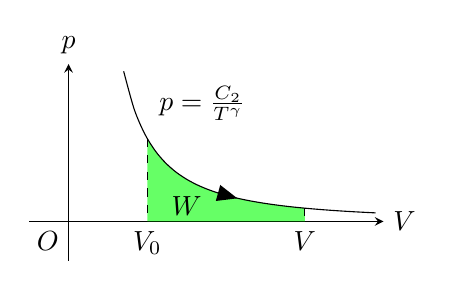
\begin{tikzpicture}
    \coordinate[label=below left:$O$] (O) at (0,0);
    \coordinate (XS) at (-0.5,0);
    \coordinate (XL) at (4,0);
    \coordinate (YS) at (0,-0.5);
    \coordinate (YL) at (0,2);
    %\coordinate[label=left:$p$] (P);
    \coordinate[label=below:$V_0$] (V0) at(1,0);
    \coordinate[label=below:$V$] (V) at (3,0);

    \draw [->, >=stealth] (XS) -- (XL) node[right]{$V$};
    \draw [->, >=stealth] (YS) -- (YL) node[above]{$p$};

    \fill[domain=1:3,smooth,green, opacity=0.6] plot(\x,\funa{\x}) -- (V) -- (V0);
    \draw[domain=0.7:3.9,smooth] plot(\x,\funa{\x});
    \draw (1.5,0.2) node{$W$};
    \draw [dashed](1,\funa{1}) -- (V0);
    \draw [dashed](3,\funa{3}) -- (V);
    \begin{feynhand}
    \propag[fer] (1.9,\funa{1.9}) to (2.1, \funa{2.1});
    \end{feynhand}
    \draw (1.7,1.5) node{$p = \frac{C_2}{T^\gamma}$};
  \end{tikzpicture}
\end{document}
